\documentclass[11pt,a4paper]{article}

\usepackage{fullpage}
\usepackage{rotating}
\usepackage{amsmath, amssymb, amsthm}
%\usepackage{mathpartir}
\usepackage{tikz}
\usepackage{verbatim}
\usepackage{url}
\usepackage{enumitem}
\usepackage{accents}

\usepackage{listings}
\usepackage{color}

\definecolor{dkgreen}{rgb}{0,0.6,0}
\definecolor{gray}{rgb}{0.5,0.5,0.5}
\definecolor{mauve}{rgb}{0.58,0,0.82}

\lstset{frame=tb,
  language=Java,
  aboveskip=3mm,
  belowskip=3mm,
  showstringspaces=false,
  columns=flexible,
  basicstyle={\small\ttfamily},
  numbers=none,
  numberstyle=\tiny\color{gray},
  keywordstyle=\color{blue},
  commentstyle=\color{dkgreen},
  stringstyle=\color{mauve},
  breaklines=true,
  breakatwhitespace=true,
  tabsize=3
}

\usetikzlibrary{trees}

\begin{document}
\title{WACC Compiler Group Project}
\author{Elyas Addo, Florian Emile, Elliot Greenwood, Jonathan King}

\maketitle

\section{The Product}
\label{sec:The Product}

\subsection{Functionality}
\label{sub:Functionality}

The front end of our compiler was functionality correct for all test files. We allowed valid WACC files through to the code generation stage, and prevented any files with errors passing through. After performing the lexical, syntactic and semantic analysis on any invalid input WACC files, the compiler would output useful errors; the line and column number followed by a message outlining the error including snippets of their code for context against the expected value.

For the code generation milestone our compiler was functionally correct for all but two test cases, both where a pair or array that is freed more than once without being reinitialised. In these cases a runtime exception should have been thrown and program exited with status code 134; however our generated code threw a null reference exception instead.

\subsection{Extensibilty}
\label{subs:Extensibilty}

The cleanliness of our design was always kept in mind whilst implementing our compiler. We wanted to make sure that our code could easily be adapted and extended in the future, perhaps with additional languages features or compiling into a different language.

As we knew we would have to do an extension, the ability to easily change the compiler was very important. To facilitate the ability to add any new features we used the visitor pattern frequently. Due to the fact all of our visit functions only knew about their context, for each new language feature it was a simple case of adding a new visit function. There were a few exceptions when we had to check for a null value of a child node in our syntax tree.

One aspect we overlooked was creating our own tree structure to represent the program. We used the parse tree provided by ANTLR which meant that if we were to replace ANTLR for a similar, but perhaps more up-to-date, tool we would have to rewrite a lot of our code base. Building an Abstract Syntax Tree (AST) of our own would mean that our methods for code generation could remain intact. We would simply need to create a class to convert from the new tool-created tree to our own AST. Having control over the tree and information stored in each node would also dramatically help within visitor methods. It could remove a lot of checks on the fields in nodes as they would provide all and only the relevant information related to a particular part of the code. 

A good deal of thought was put into the possibility of changing the output assembly language. In a few years ARM11 may not be desirable; by extracting all the ARM11 specific code into it's own package, changing the output language would simply involve swapping that package for, say, a x86 package. Our code would not change as the instruction factory would simply return x86 instructions as opposed to ARM11 instructions. Additionally we could add support for generating LLVM intermediate representation (IR), and let LLVM to perform code generation.

\section{The Project Management}
\label{sec:The Project Management}

\subsection{Group Structure}
\label{sub:Group Structure}

We split into pairs to program for larger sections of feature implementations. For smaller sections, members would work independently.

Pair programming made catching simple mistakes easier and forced us to discuss design choices, logical processes and other decisions before implementing them, leading to many fewer errors to debug. The independent work for smaller sections meant we were able to get more work done in a smaller amount of time and not have a member sat idle for trivial implementations.

\subsection{Use of Project Management Tools}
\label{sub:Use of Project Management Tools}

To help organise the team we used a few project management tools and continuous integration platforms.

\subsubsection{Maven}
\label{subs:Maven}

We used Maven to structure our project. Using Maven meant we didn't have to take care of dependencies, such as ANTLR, the make process was also simplified as using the command \texttt{mvn package} would generate the ANTLR java files, test our code using the unit tests we had created and package our code, including the dependencies, into a .jar file.


\subsubsection{Git and Github}
\label{subs:Git and Github}

We used Git and Github as our chosen version control. We utilised branches to keep features and sub features seperate, then use pull requests to merge all of our features together. Below is a diagram showing the main branches for our project.

\tikzstyle{every node}=[draw=black,thick,anchor=west]
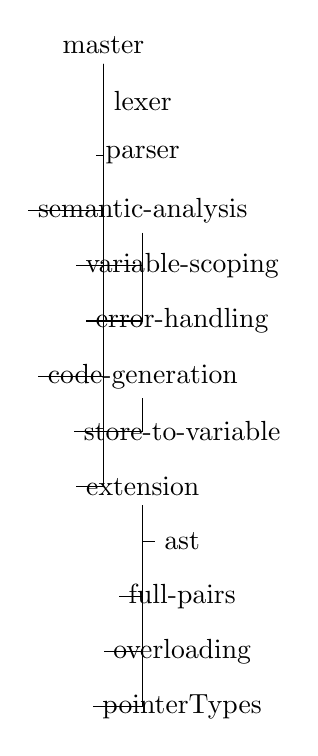
\begin{tikzpicture}[%
  grow via three points={one child at (0.5,-0.7) and
  two children at (0.5,-0.7) and (0.5,-1.4)},
  edge from parent path={(\tikzparentnode.south) |- (\tikzchildnode.west)}]

  \node {master}
    child { node {lexer}}
    child { node {parser}}
    child { node {semantic-analysis}
      child { node {variable-scoping}}
      child { node {error-handling}}
    }
    child [missing] {}
    child [missing] {}
    child { node {code-generation}
      child { node {store-to-variable}}
    }
    child [missing] {}
    child { node {extension}
      child { node {ast}}
      child { node {full-pairs}}
      child { node {overloading}}
      child { node {pointerTypes}}
    };
\end{tikzpicture}

Github provided us with Issues which we used to keep track of current bugs and enhancements we wanted to implement. It also gave us the option to assign that issue to a member of our team.

Our git commit messages on the whole were quite short and vague, though the style of our messages were on the correct path. Where possible we would style our commit messages to include the people who were working on the commit, an instruction that would tell the reader what the commit should do (i.e. Implement x instead of Implemented x).

\subsubsection{Travis CI}
\label{subs:Travis}
We used Travis, a continuous integration service, which ran tests on our code after every push and before merging pull requests. This integration with Github meant we would never merge a pull request in the event of our commit failing the unit tests.\\
Automated testing gave us confidence that our code was correct

as you can always prove that your most important features still work as you expect - documented history

as the tests were run on a remote machine it meant, which could take a few minutes to run - get an email/slack notification on test success/failure.

A side effect of , which created a new virtual machine  

Not useful in, but useful in backend to prevent regression of previous milestones. - will get more useful with time.

Travis has proven more useful as the project progressed, 

In the branch \texttt{travis-emulator} we experimented with, and successfully, this is certainly to remove dependance on LabTS - however decided to spend time in other areas - more useful at the time.

\subsection{Slack}
\label{sub:Slack}
Our communication platform of choice was Slack, we liked the features is boasted such as channels, intergrations and snippets, which can be non-existent to contrived in other apps such as Facebook and Email.

Channels meant we could have a seperate section for each milestone, as well as a general channel for of topic conversation. This kept all of our WACC messages in one place that was not polluted by other conversations.

Integrations were really useful, the two intergrations we used the most were Github and Travis. Every time we made a commit, a new branch, an issue, assigned an issue to someone, etc. it would be automatically posted on the relevant Slack channel so everyone could read it. This stopped the need for people to ask when something had been pushed, and meant we could easily reference a certain commit. One intergration we would have liked to have used more is Wunderlist, that way we could create a centralised list of all the tasks we had todo instead of having our own lists.

Snippets were useful if we needed to send each other short pieces of code that did not warrant a commit. We would also create snippets containing the key errors produced from running tests so everyone could see what the stack trace and actual output was without us having to run the tests n times.

\subsection{What Would We Do Differently?}
\label{sub:What Would We Do Differently?}

If we were to do this lab exercise again, we would include the creation of an AST form the start. The AST could be built as soon as parsing the input file is complete. If this building process were to occur at this point in compilation, types would be created at the same time. This would remove the need for a separate visitor to create types when building the symbol table.

In terms of compiler outputs, we would like to create more user-friendly error messages. This includes changing the ANTLR error messages produced in lexical and syntactic analysis not to display a set of possible characters, but instead information on how that particular program construct should be written.

As an improvement to our work practice, we would Test Driven Development (TDD) on all aspects of our compiler. We did use TDD for parts of our compiler, however, the visitors made this slightly tricky since we were forced to use black-box testing to check the overall functionality of the class with regards to a particular WACC programming construct.

\section{The Design Choices}
\label{sec:The Design Choices}

\subsection{Visitor}
\label{sub:Visitor}
We used the visitor pattern four times in our project. It was used in front end to create the WACC language types and add them to our symbol table. It was also used for creating the symbol table structure and for checking validity of types for expressions, statements and other constructs with respect to the WACC specification. Back end used a visitor as well to generate the correct assembly code. As previously mentioned, this pattern allows easier inclusion of language features by adding a new visit method. Without this we would have to use large if statements and many switch cases, increasing for every new parser rule. This is especially undesirable as running \texttt{make} will rebuild the ANTLR files thereby removing any custom code we had added.

\subsection{Factory}
\label{sub:Factory}
To create our instructions we used the Factory pattern to produce all the different types. This way, instead of creating a class for each type of instruction, we return an anonymous class that implements the interface \texttt{Instruction}. We used Java 8 lambdas to create the instructions as there is only one method \texttt{printInstruction}. This gave a clean and minimal solution to creating all of our instructions.

\subsection{Command Line Interface Seperation}
\label{sub:Command Line Interface Seperation}
We used redirection in our compile script to allow our input file to be passed in as the System.in, this means our compiler does not need to know about files, it can just take the file contents and create an input stream.

\section{Beyond the Specification}
\label{sec:Beyond the Specification}
For our extension, we chose to extend the WACC language. 

\begin{enumerate}
	\item Function Overloading\newline
	Functions can now have the same name as long as they have different lists of parameters. These overloaded functions can have different return types since they are, in essence, different functions. Pairs in WACC are treated as Objects in Java with generic parameters are treated. This mean that you cannot have a function \texttt{f(pair(int, char))} and another function \texttt{pair(bool, string)} since they have the same erasure.
	
	\item Pointer Types\newline
	The WACC language now has a C-style pointer type. We can now access a variable using its memory address using \texttt{*} followed by the pointer name. To get the address of a variable we created an address operator: \texttt{\&} (we need this to initialise pointers).
	
	\item \texttt{if} statements with no \texttt{else} case\newline
	If statements without an else case are now valid.
	
	\item Optional \texttt{;} at the end of a list of statements
	Most programming languages which use \texttt{;} to separate different statements. Forcing the final statement in a particular code block to have no following \texttt{;} may become an irritating syntax rule to follow. We have removed this rule to allow more comfortable coding and a more consistent style.
	
	\item Full Pairs\newline
	The WACC language now has a full typing system for pairs. This means that no type information is lost for nested pairs. 
	
\end{enumerate}

We wrote new test files in order to assess whether or not the language extension implementations behaved as intended. Since we also wanted to ensure that these implementations did not brake any of the original specification elements, we adapted out test scripts to run all previous tests and new tests. Due to the nature of some of the language extensions, 2 previous test cases failed. These were \texttt{ifNoelse.wacc} and \texttt{extraSeq.wacc}.

If we had more time, we would have liked to implement some optimisations on our assembly code such as efficient register allocation and array-bound analysis. We were also quite keen on making WACC object-oriented - implementing classes, inheritance, and advanced features of classes such as multiple-inheritance, overriding and class constructors.

\end{document}
